%%
%% Automatically generated file from DocOnce source
%% (https://github.com/hplgit/doconce/)
%%
%%


%-------------------- begin preamble ----------------------

\documentclass[%
oneside,                 % oneside: electronic viewing, twoside: printing
final,                   % draft: marks overfull hboxes, figures with paths
10pt]{article}

\listfiles               %  print all files needed to compile this document

\usepackage{relsize,makeidx,color,setspace,amsmath,amsfonts,amssymb}
\usepackage[table]{xcolor}
\usepackage{bm,ltablex,microtype}

\usepackage[pdftex]{graphicx}

\usepackage{fancyvrb} % packages needed for verbatim environments

\usepackage[T1]{fontenc}
%\usepackage[latin1]{inputenc}
\usepackage{ucs}
\usepackage[utf8x]{inputenc}

\usepackage{lmodern}         % Latin Modern fonts derived from Computer Modern

% Hyperlinks in PDF:
\definecolor{linkcolor}{rgb}{0,0,0.4}
\usepackage{hyperref}
\hypersetup{
    breaklinks=true,
    colorlinks=true,
    linkcolor=linkcolor,
    urlcolor=linkcolor,
    citecolor=black,
    filecolor=black,
    %filecolor=blue,
    pdfmenubar=true,
    pdftoolbar=true,
    bookmarksdepth=3   % Uncomment (and tweak) for PDF bookmarks with more levels than the TOC
    }
%\hyperbaseurl{}   % hyperlinks are relative to this root

\setcounter{tocdepth}{2}  % levels in table of contents

% Tricks for having figures close to where they are defined:
% 1. define less restrictive rules for where to put figures
\setcounter{topnumber}{2}
\setcounter{bottomnumber}{2}
\setcounter{totalnumber}{4}
\renewcommand{\topfraction}{0.95}
\renewcommand{\bottomfraction}{0.95}
\renewcommand{\textfraction}{0}
\renewcommand{\floatpagefraction}{0.75}
% floatpagefraction must always be less than topfraction!
% 2. ensure all figures are flushed before next section
\usepackage[section]{placeins}
% 3. enable begin{figure}[H] (often leads to ugly pagebreaks)
%\usepackage{float}\restylefloat{figure}

% prevent orhpans and widows
\clubpenalty = 10000
\widowpenalty = 10000

% --- end of standard preamble for documents ---


% insert custom LaTeX commands...

\raggedbottom
\makeindex
\usepackage[totoc]{idxlayout}   % for index in the toc
\usepackage[nottoc]{tocbibind}  % for references/bibliography in the toc

%-------------------- end preamble ----------------------

\begin{document}

% matching end for #ifdef PREAMBLE

\newcommand{\exercisesection}[1]{\subsection*{#1}}


% ------------------- main content ----------------------



% ----------------- title -------------------------

\thispagestyle{empty}

\begin{center}
{\LARGE\bf
\begin{spacing}{1.25}
Project 5, deadline  December 9, 2016
\end{spacing}
}
\end{center}

% ----------------- author(s) -------------------------

\begin{center}
{\bf Astronomy project, $N$-body simulation of an open galactic cluster${}^{}$} \\ [0mm]
\end{center}

\begin{center}
% List of all institutions:
\end{center}
    
% ----------------- end author(s) -------------------------

% --- begin date ---
\begin{center}
Fall semester 2016
\end{center}
% --- end date ---

\vspace{1cm}


\subsection*{Theoretical background and description of the system}

The goal of this project is to develop a code that can perform
simulations of an open cluster using Newtonian gravity. 
This project is inspired by an article by
\href{{http://dx.doi.org/10.1063/1.3462740}}{M. Joyce and co-workers}, see also the references below.  When solving this
project, we recommend downloading this article. It is a good companion
to understand the physics discussed here.
This project requires a good  background in cosmology and
astrophysics. The project can be seen as a continuation of project 3 and we will use again
the Velocity Verlet algorithm. 

We will try to build a simple model of an open
cluster, as done by \href{{http://dx.doi.org/10.1063/1.3462740}}{M. Joyce and co-workers}. An
open cluster is a group of up to a few thousand gravitationally bound
stars created from the collapse of a molecular cloud. This collapse
leads to a flurry of star formation. Open clusters are usually found
in the arms of spiral galaxies, or in irregular galaxies. Since stars
in an open cluster have roughly the same age, and are made from the
same material, they are interesting in the study of stellar evolution,
since many of the variable parameters we have when comparing two stars
are kept constant.

Once open clusters are formed they gradually dissipate as members get
ejected from the cluster due to random collisions, this means that
open clusters generally last only a few hundred million years. In
the figure here we see the Hertzsprung-Russell diagrams for two open
clusters.


\begin{figure}[!ht]  % 
  \centerline{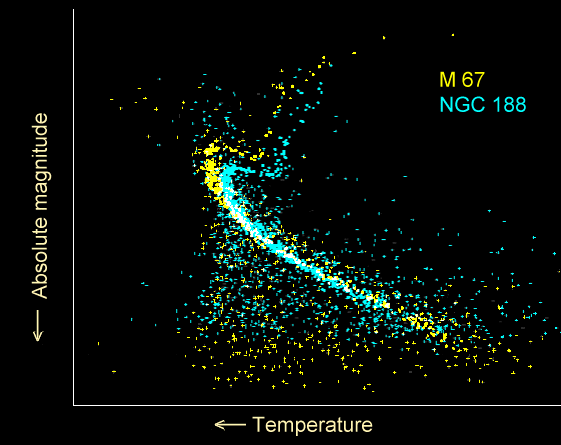
\includegraphics[width=1.0\linewidth]{open_cluster_hr_diagram_ages.png}}
  \caption{
  Hertzsprung-Russell diagrams for two open clusters, M67 and   NGC 188. We see that most of the stars are on the main sequence. In   the older cluster, NGC 188, we see that the heaviest stars are just   now leaving the main sequence, while the younger cluster, M67.
  }
\end{figure}
%\clearpage % flush figures 


We will study a simple model for how an open cluster is made from
the gravitational collapse and interaction among a large number of
stars. We want to study this collapse, and the statistical properties
of the collapsed system.
We will simulate what is called a
\emph{cold collapse}, this means that we start the particles with little
or no initial velocity. You will also find it useful to start with the code you developed in project 3.


\paragraph{Project 5a): Extension of project 3.}
Extend your code from project 3 to an arbitrary number of particles, $N$,
  starting with a uniform (random) distribution within a sphere of a
  given radius $R_0$. Start the particles at rest, with masses
  randomly distributed by a Gaussian distribution around ten solar
  masses with a standard deviation of one solar mass. Use solar masses
  and light years as units of mass and length and make your equations dimensionless.
This function is included below and  can be used to generate 
random numbers which follow a Gaussian (or normal) distribution.  Alternatively, you can use 
the \emph{random} class in c++ and generate random numbers according to the normal distribution.

How large time steps are required given $R_0 = 20$ ly
(light years), and  $N = 100$? Do we have any units of time that fit
this timescale?   
In the limit where $N \rightarrow \infty$, keeping $\rho_0$ constant,
we get a continuous fluid. In this case the system collapses into a
singularity at a finite time $\tau_{\mathrm{crunch}} = \sqrt{\frac{3\pi}{32G\rho_0}}$. 

Why do we not observe this singularity in our model? Use
$\tau_{\mathrm{crunch}}$ as the unit of time, and find $G$ in these units ($G$
will become a function of the number of particles $N$, and the average
mass of the particles, $\mu$).

\paragraph{Project 5b): Time to reach equilibrium.}
Run the system for a few $\tau_{\mathrm{crunch}}$. Save the positions
  of the particles at different times to file. Does the system
  reach an equilibrium? How long time does this take?


\paragraph{Project 5c): Kinetic and potential energy.}
Make a function that calculates the kinetic and potential
  energy of the system. Is the energy conserved? Some of the
  particles are ejected from the system, how can we identify these
  particles from the energies we have calculated? How much of the
  energy of the system is taken away by particle ejection? How does
  this change with different values of $N$? Are there still particles
  being ejected after the system reaches equilibrium?

\paragraph{Project 5d): Numerical instabilities.}
We will now introduce a smoothing function to take care of
  the numerical instability that arises when two of the particles come
  very close. There are a lot of ways of inserting such a smoothing, but
  we will just look at a very simple one. We will modify the Newtonian
  force law to make it finite at short ranges

\begin{equation*} 
F_{mod} = -\frac{GM_1M_2}{r^2 + \epsilon^2}.
\end{equation*}

The parameter $\epsilon$ is a \emph{small} real constant. What should the value of this parameter be? Try out different values (which one gives you the best energy conservation?). Can we justify this correction to the pure Newtonian force by noting that our particles do not represent actual point particles
but rather mass distributions of some finite extent? Does the addition
of this correction change any of the results from the previous exercise?


\paragraph{Project 5e): Test of the virial theorem.}
Now we will look at the particles that are bound (not ejected). 
What is the distribution of potential and kinetic energy?

The virial theorem says that for a bound gravitational system in
equilibrium we have

\begin{equation*}
2\langle K\rangle = -\langle V \rangle,
\end{equation*}
where $\langle K\rangle$
is the average (over time) kinetic energy of the system and $ \langle V
\rangle$ is the average potential energy. 

By the ergodic hypothesis we can take an ensemble 
average (average over a large system) instead of the time average. 

Are your results consistent with the virial theorem? 


\paragraph{Project 5f): Density of particles.}
Try to plot the radial density of the particles (the particle density as a function of radius) in the
  equilibrium state. How would you extract such an information from your calculations? (Hint: make a histogram for the radial
particle density) What is the average distance? What is the
  standard deviation? Plot the radial distribution of particles.

Run the code for different number of initial particles, keeping the
total mass constant. The interpretation of one particle as one or a few stars will not be useful any more when you increase the number of particles beyond a few thousand, however the analysis of gravitationally bound systems of many particles have much broader applications than cold collapse of open clusters, so the results are still highly relevant. What is the average distance from the centre of the cluser as a function of $N$?

The radial distribution of particles in this kind of cold collapse can often be fit very well with the simple expression

\begin{equation*} 
n(r) = \frac{n_0}{\left(1 +\left(\frac{r}{r_0}\right)^4\right)}.
\end{equation*}
Try to fit your data to this curve, what is the value $n_0$ and $r_0$? Can you find how these values depend on N?

How many particles can you simulate?

Compare your results with those found in  \href{{http://dx.doi.org/10.1063/1.3462740}}{M. Joyce and co-workers}.

If you want, you can also compare your results to the well-known Navarro-Frenk-White profile

\begin{equation*} 
\rho(r) = \frac{\rho_0}{\frac{r}{r_0}\left(1 +\frac{r}{r_0}\right)^2}.
\end{equation*}
Does this give a  better fit?


\paragraph{References.}
\begin{enumerate}
\item \href{{http://dx.doi.org/10.1063/1.3462740}}{M. Joyce, B. Marcos, and F. Sylos Labini, Cold uniform spherical collapse revisited, AIP Conf. Proc. 1241, 955 (2010)}. See also \href{{http://arxiv.org/abs/1011.0614}}{arXiv1011.0614 (2011)}.

\item P. J. E. Peebles, \emph{The Large-Scale Structure of the Universe}, Princeton University Press, 1980. See also C. Payne-Gaposchkin,  \emph{Stars and clusters}, (Cambridge, Harvard University Press, 1979).

\item A. Friedman,  On the Curvature of Space,  General Relativity and Gravitation 31,  1991 (1999)":"http://link.springer.com/article/10.1023%2FA%3A1026751225741".
\end{enumerate}

\noindent
\paragraph{Function for Gaussian random numbers.}
\begin{verbatim}
// ran2 for uniform deviates, initialize with negative seed.
double ran2(long *);

// function for gaussian random numbers
double gaussian_deviate(long *);

/*
** The function 
**         ran2()
** is a long periode (> 2 x 10^18) random number generator of 
** L'Ecuyer and Bays-Durham shuffle and added safeguards.
** Call with idum a negative integer to initialize; thereafter,
** do not alter idum between sucessive deviates in a
** sequence. RNMX should approximate the largest floating point value
** that is less than 1.
** The function returns a uniform deviate between 0.0 and 1.0
** (exclusive of end-point values).
*/

#define IM1 2147483563
#define IM2 2147483399
#define AM (1.0/IM1)
#define IMM1 (IM1-1)
#define IA1 40014
#define IA2 40692
#define IQ1 53668
#define IQ2 52774
#define IR1 12211
#define IR2 3791
#define NTAB 32
#define NDIV (1+IMM1/NTAB)
#define EPS 1.2e-7
#define RNMX (1.0-EPS)

double ran2(long *idum)
{
  int            j;
  long           k;
  static long    idum2 = 123456789;
  static long    iy=0;
  static long    iv[NTAB];
  double         temp;

  if(*idum <= 0) {
    if(-(*idum) < 1) *idum = 1;
    else             *idum = -(*idum);
    idum2 = (*idum);
    for(j = NTAB + 7; j >= 0; j--) {
      k     = (*idum)/IQ1;
      *idum = IA1*(*idum - k*IQ1) - k*IR1;
      if(*idum < 0) *idum +=  IM1;
      if(j < NTAB)  iv[j]  = *idum;
    }
    iy=iv[0];
  }
  k     = (*idum)/IQ1;
  *idum = IA1*(*idum - k*IQ1) - k*IR1;
  if(*idum < 0) *idum += IM1;
  k     = idum2/IQ2;
  idum2 = IA2*(idum2 - k*IQ2) - k*IR2;
  if(idum2 < 0) idum2 += IM2;
  j     = iy/NDIV;
  iy    = iv[j] - idum2;
  iv[j] = *idum;
  if(iy < 1) iy += IMM1;
  if((temp = AM*iy) > RNMX) return RNMX;
  else return temp;
}
#undef IM1
#undef IM2
#undef AM
#undef IMM1
#undef IA1
#undef IA2
#undef IQ1
#undef IQ2
#undef IR1
#undef IR2
#undef NTAB
#undef NDIV
#undef EPS
#undef RNMX

// End: function ran2()



// random numbers with gaussian distribution
double gaussian_deviate(long * idum)
{
  static int iset = 0;
  static double gset;
  double fac, rsq, v1, v2;

  if ( idum < 0) iset =0;
  if (iset == 0) {
    do {
      v1 = 2.*ran2(idum) -1.0;
      v2 = 2.*ran2(idum) -1.0;
      rsq = v1*v1+v2*v2;
    } while (rsq >= 1.0 || rsq == 0.);
    fac = sqrt(-2.*log(rsq)/rsq);
    gset = v1*fac;
    iset = 1;
    return v2*fac;
  } else {
    iset =0;
    return gset;
  }
} // end function for gaussian deviates

\end{verbatim}

\subsection*{Introduction to numerical projects}

Here follows a brief recipe and recommendation on how to write a report for each
project.

\begin{itemize}
  \item Give a short description of the nature of the problem and the eventual  numerical methods you have used.

  \item Describe the algorithm you have used and/or developed. Here you may find it convenient to use pseudocoding. In many cases you can describe the algorithm in the program itself.

  \item Include the source code of your program. Comment your program properly.

  \item If possible, try to find analytic solutions, or known limits in order to test your program when developing the code.

  \item Include your results either in figure form or in a table. Remember to        label your results. All tables and figures should have relevant captions        and labels on the axes.

  \item Try to evaluate the reliabilty and numerical stability/precision of your results. If possible, include a qualitative and/or quantitative discussion of the numerical stability, eventual loss of precision etc.

  \item Try to give an interpretation of you results in your answers to  the problems.

  \item Critique: if possible include your comments and reflections about the  exercise, whether you felt you learnt something, ideas for improvements and  other thoughts you've made when solving the exercise. We wish to keep this course at the interactive level and your comments can help us improve it.

  \item Try to establish a practice where you log your work at the  computerlab. You may find such a logbook very handy at later stages in your work, especially when you don't properly remember  what a previous test version  of your program did. Here you could also record  the time spent on solving the exercise, various algorithms you may have tested or other topics which you feel worthy of mentioning.
\end{itemize}

\noindent
\subsection*{Format for electronic delivery of report and programs}

The preferred format for the report is a PDF file. You can also use DOC or postscript formats or as an ipython notebook file.  As programming language we prefer that you choose between C/C++, Fortran2008 or Python. The following prescription should be followed when preparing the report:

\begin{itemize}
  \item Use Devilry to hand in your projects, log in  at  \href{{http://devilry.ifi.uio.no}}{\nolinkurl{http://devilry.ifi.uio.no}} with your normal UiO username and password and choose either 'fys3150' or 'fys4150'. There you can load up the files within the deadline.

  \item Upload \textbf{only} the report file!  For the source code file(s) you have developed please provide us with your link to your github domain.  The report file should include all of your discussions and a list of the codes you have developed.  Do not include library files which are available at the course homepage, unless you have made specific changes to them.

  \item In your git repository, please include a folder which contains selected results. These can be in the form of output from your code for a selected set of runs and input parametxers.

  \item In this and all later projects, you should include tests (for example unit tests) of your code(s).

  \item Comments  from us on your projects, approval or not, corrections to be made  etc can be found under your Devilry domain and are only visible to you and the teachers of the course.
\end{itemize}

\noindent
Finally, 
we encourage you to work two and two together. Optimal working groups consist of 
2-3 students. For this specific report you can  hand in a common report.














% ------------------- end of main content ---------------

\end{document}

